 
\chapter{Выбор рациональной конструкции}
Как было отмечено в разделе \ref{sec:ndsResults}, одним из проблемных с мест конструкции гипотетического БПЛА, с точки зрения прочности, является силовой элемент конструкции, обеспечивающий основное крепление к центроплану хвостовой части, в которой находится двигатель. В целях нахождения наиболее эффективной в весовом отношении конфигурации силовой структуры гипотетического БПЛА в работе был проведен сравнительный анализ различных вариантов исполнения данного элемента. Для проведения этого анализа были выбраны три варианта конструкции, представленные на схемах на Рис.\ref{fig:variants_plain} и изображениях МКЭ-моделей на Рис.\ref{fig:variants_mke}. Для анализа была использована модель, описанная в разделе \ref{sec:creationOfOneModel} и две модели, созданные на её основе. Все три модели были адаптированы с учетом выводов, которые будут получены в разделе \ref{sec:optimalMKESize}.  

\begin{figure}[H]
\centering
\captionsetup{justification=centering}
\begin{subfigure}[b]{0.32\textwidth}
\centering
	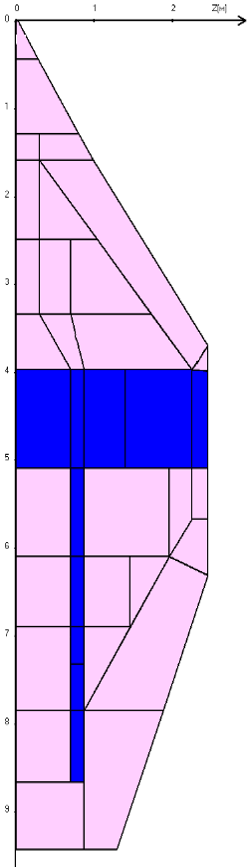
\includegraphics[width=0.3\textwidth]{variants/1_plain}
	\caption{Вариант 1}
\end{subfigure}
\hspace{\fill}
\begin{subfigure}[b]{0.32\textwidth}
\centering
	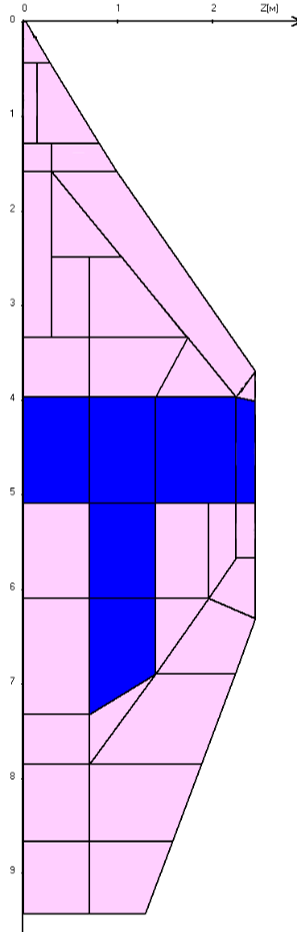
\includegraphics[width=0.3\textwidth]{variants/2_plain}
	\caption{Вариант 2}
\end{subfigure}
\hspace{\fill}
\begin{subfigure}[b]{0.32\textwidth}
\centering
	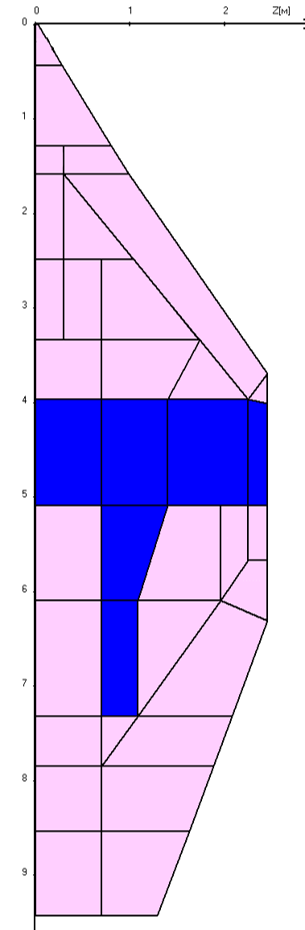
\includegraphics[width=0.3\textwidth]{variants/3_plain}
	\caption{Вариант 3}
\end{subfigure}
\hspace{\fill}
\caption{Схематичные изображения центроплана и соединительной конструкции на виде ``в плане'' половины фюзеляжа }
\label{fig:variants_plain}
\end{figure}	


\begin{figure}[H]
\centering
\begin{subfigure}[b]{0.32\textwidth}
	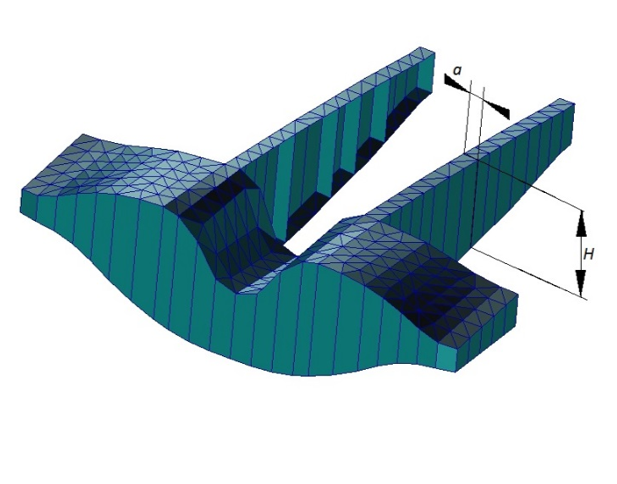
\includegraphics[width=\textwidth]{variants/1_mke}		\caption{Вариант 1}
	\label{fig:variants_mke:1}
\end{subfigure}
\hspace{\fill}
\begin{subfigure}[b]{0.32\textwidth}
	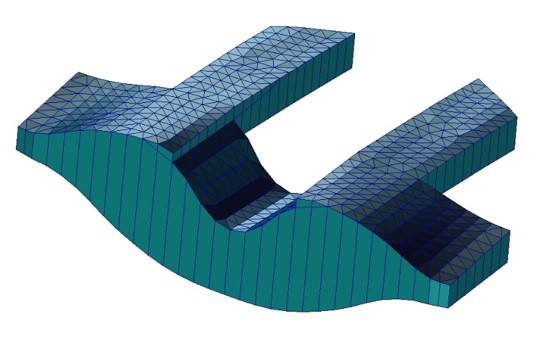
\includegraphics[width=\textwidth]{variants/2_mke}
		\caption{Вариант 2}
		\label{fig:variants_mke:2}
\end{subfigure}
\hspace{\fill}
\begin{subfigure}[b]{0.32\textwidth}
	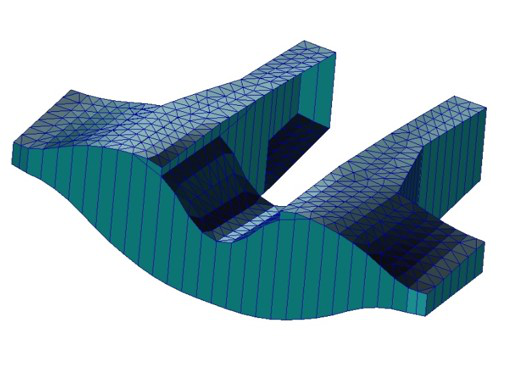
\includegraphics[width=\textwidth]{variants/3_mke}
		\caption{Вариант 3}
		\label{fig:variants_mke:3}
\end{subfigure}
\hspace{\fill}
\caption{Виды МКЭ-моделей центроплана и соединительного элемента}
\label{fig:variants_mke}
\end{figure}	



\section{Определение рациональной дискретности модели}
\label{sec:optimalMKESize}

В целях обеспечения точности расчета было проведено исследование зависимости 
НДС гипотетической модели БПЛА, представленной в разделе \ref{sec:creationOfOneModel} (именуемой далее базовой моделью), от максимального характерного размера конечных элементов, используемых в модели. 

Решение поставленной задачи заключается в проектировании трех вариантов первичной конструкции БПЛА, отличающихся друг от друга конструктивно-силовой схемой для части планера, и проведении сравнительного весового анализа для этих вариантов. Для корректного сравнения результатов проектирования различных конструкций необходимо, чтобы уровень точности результатов прочностных расчетов для этих конструкций был одинаковым. Поскольку точность прочностных расчетов напрямую зависит от размеров конечных элементов (от густоты КЭ-сетки) в модели исследуемой конструкции, то наиболее простым способом выполнить это условие являлось использование КЭ-сетки с максимально возможной густотой. Однако, процесс оптимизации моделей такой большой размерности не представлялся возможным в рамках проводимых исследований. Поэтому обеспечение достаточной точности решений для различных вариантов конструкции заключался в определении для каждого из этих вариантов максимального размера конечных элементов, при последовательном уменьшении которого максимальные напряжения в критических точках, влияющие на прочность конструкции, изменялись не более, чем на заданную величину (в данной задаче использовалась относительная величина 5%).


С помощью программного комплекса ``Conver'', на основе базовой модели, для каждого из исследуемых вариантов конструкции было построено 7 моделей БПЛА, отличающихся лишь максимальным размером конечных элементов, используемых при построении модели. На Рис.\ref{fig:discreteness} представлены некоторые из построенных моделей. Для сравнительного анализа моделей были выбраны четыре точки, в которых, в соответствии с результатами, полученными в разделе \ref{sec:ndsResults}, обнаруживались наибольшие напряжения (Рис.\ref{fig:criticalPointsBoth}). Путем расчета полученных моделей с помощью программного продукта MSC.Nastran были получены величины напряжений в этих четырех точках для каждой модели.


\begin{figure}[ht]
\captionsetup{justification=centering}
\centering
	\begin{subfigure}[b]{0.8\textwidth}
	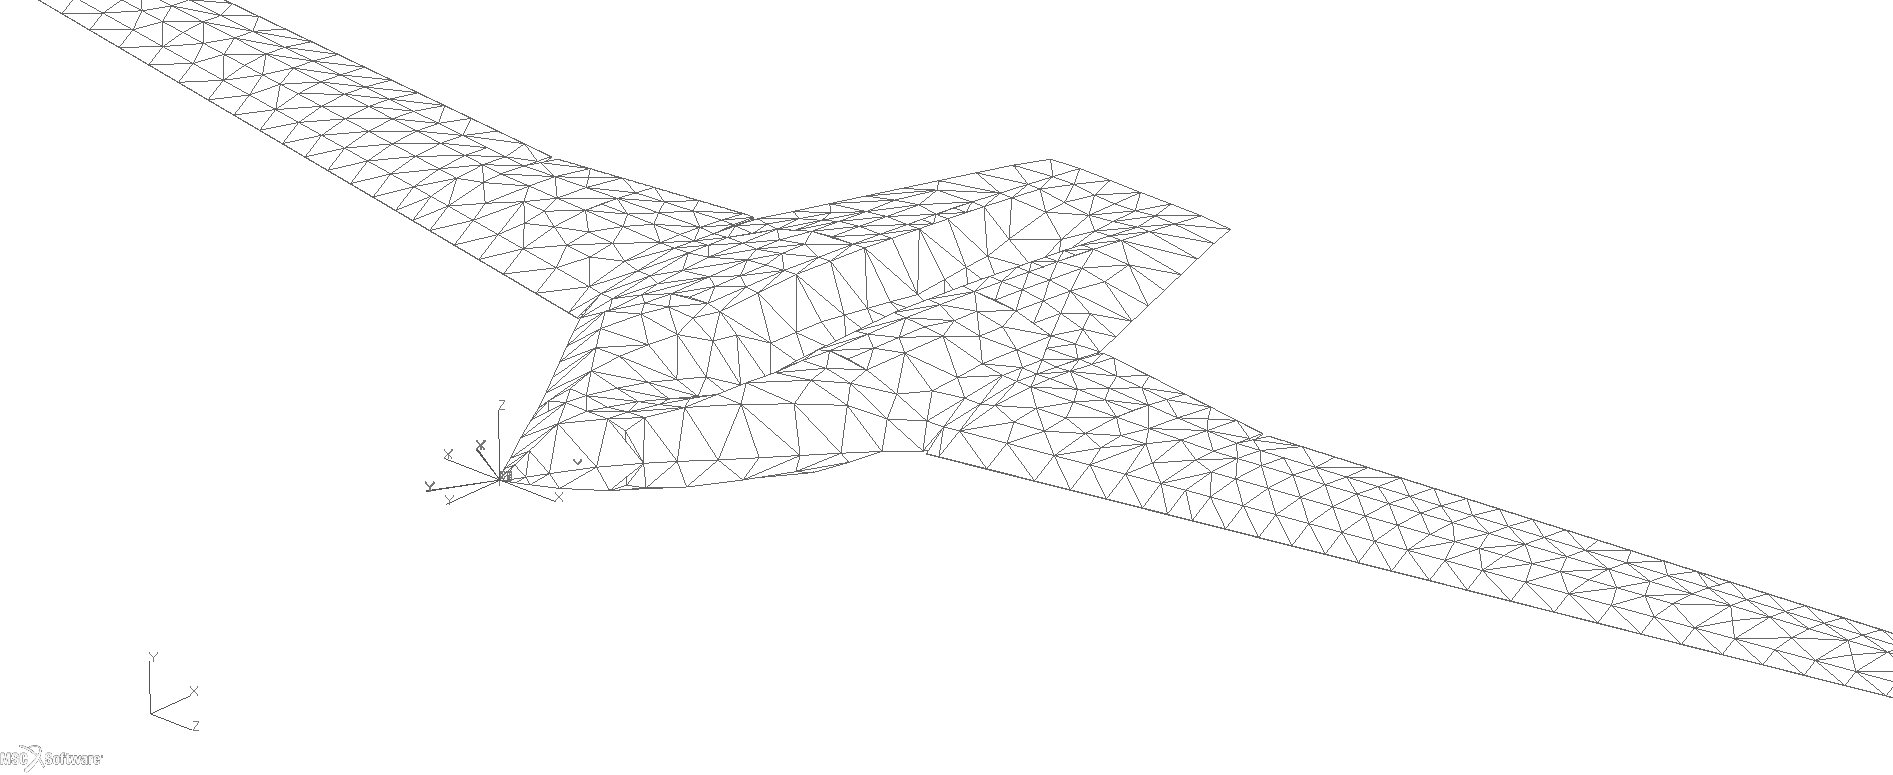
\includegraphics[width=0.98\textwidth]{discreteness/0_4}
	\caption{$L_\text{КЭ} = 0.4см$}
	\label{fig:discr:0_4}
	\end{subfigure}
	\begin{subfigure}[b]{0.8\textwidth}
	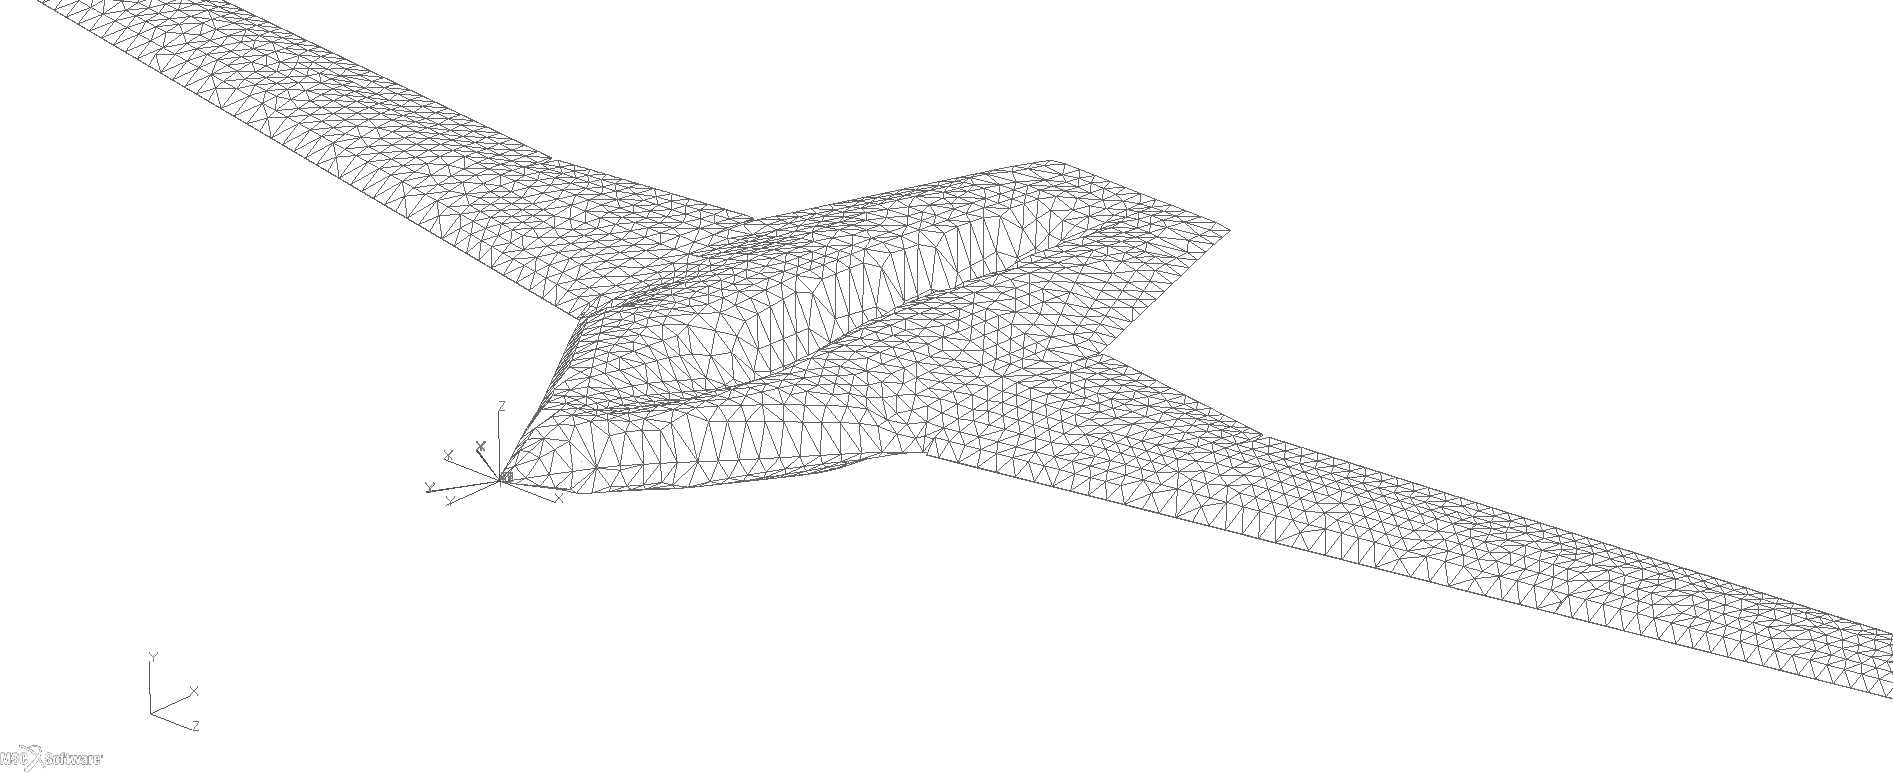
\includegraphics[width=0.98\textwidth]{discreteness/0_2}
	\caption{$L_\text{КЭ} = 0.2см$}
	\label{fig:discr:0_2}
	\end{subfigure}
	\begin{subfigure}[b]{0.8\textwidth}
	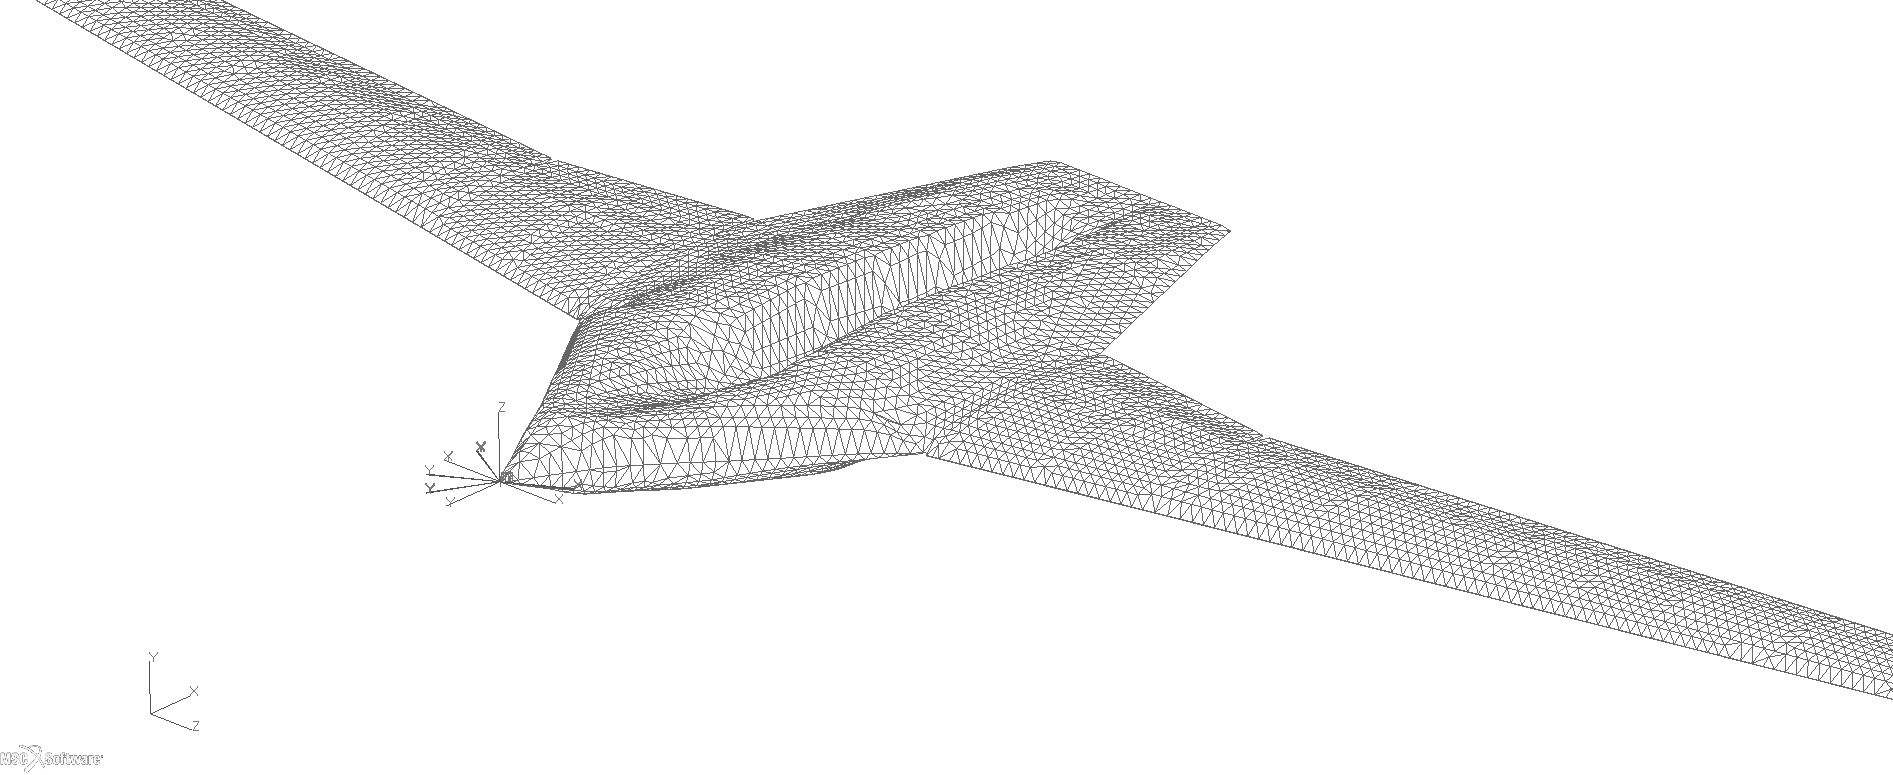
\includegraphics[width=0.98\textwidth]{discreteness/0_13}
	\caption{$L_\text{КЭ} = 0.13см$}
	\label{fig:discr:0_13}
	\end{subfigure}
\caption{Изображения МКЭ-моделей гипотетического БПЛА, построенных с использованием различных характерных размеров конечного элемента}
\label{fig:discreteness}
\end{figure}

%Нужно пересчитывать график

\begin{figure}[ht]
	\centering
	\begin{subfigure}[b]{0.47\textwidth}
	\def\svgwidth{\textwidth}
	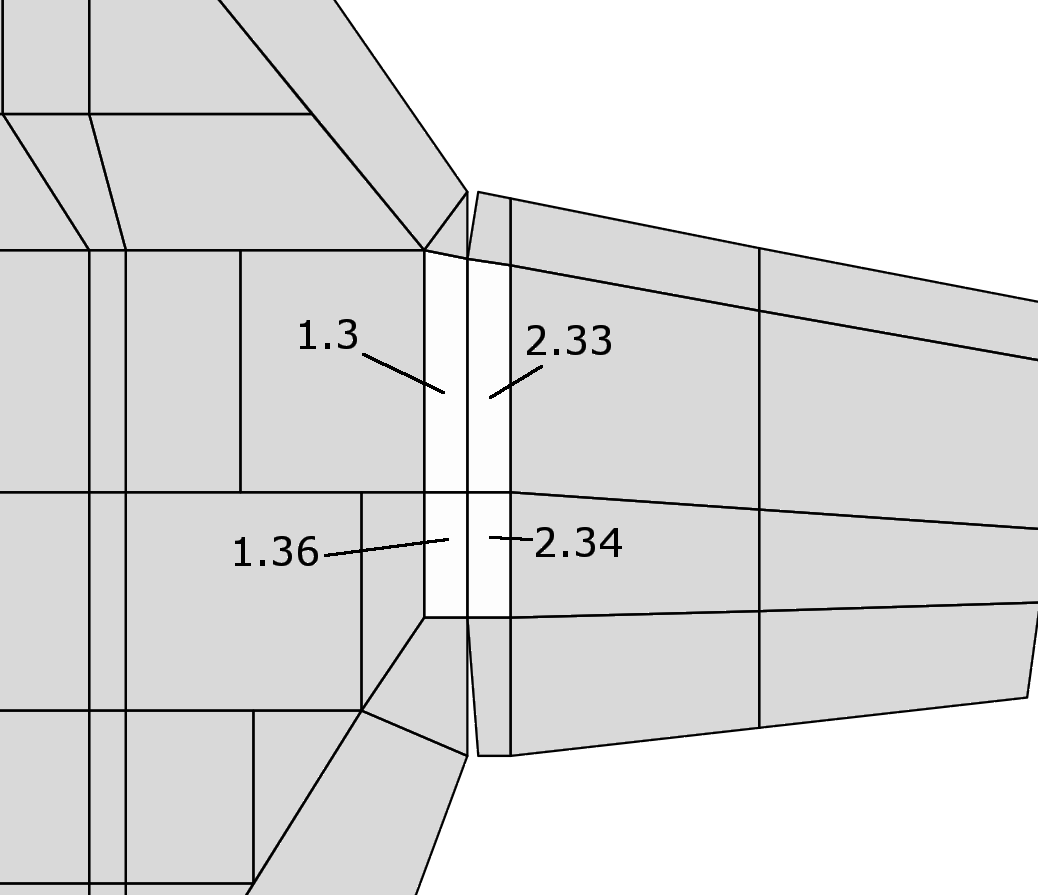
\includegraphics[width=\textwidth]{RootOfWingWithSelectedPartsBW}
	\caption{Схематичное изображение вида сверху в месте стыка правого крыла и фюзеляжа}
	\label{fig:WingRootPlain}	
	\end{subfigure}
	\begin{subfigure}[b]{0.47\textwidth}
	\def\svgwidth{\textwidth}
	\input{figures/criticalPoints.pdf_tex}
	\caption{Вид НДС гипотетической конструкции БПЛА сверху}
	\label{fig:criticalPoints}	
	\end{subfigure}
\caption{Изображения расположения критических точек}
\label{fig:criticalPointsBoth}
\end{figure}

%\centering
%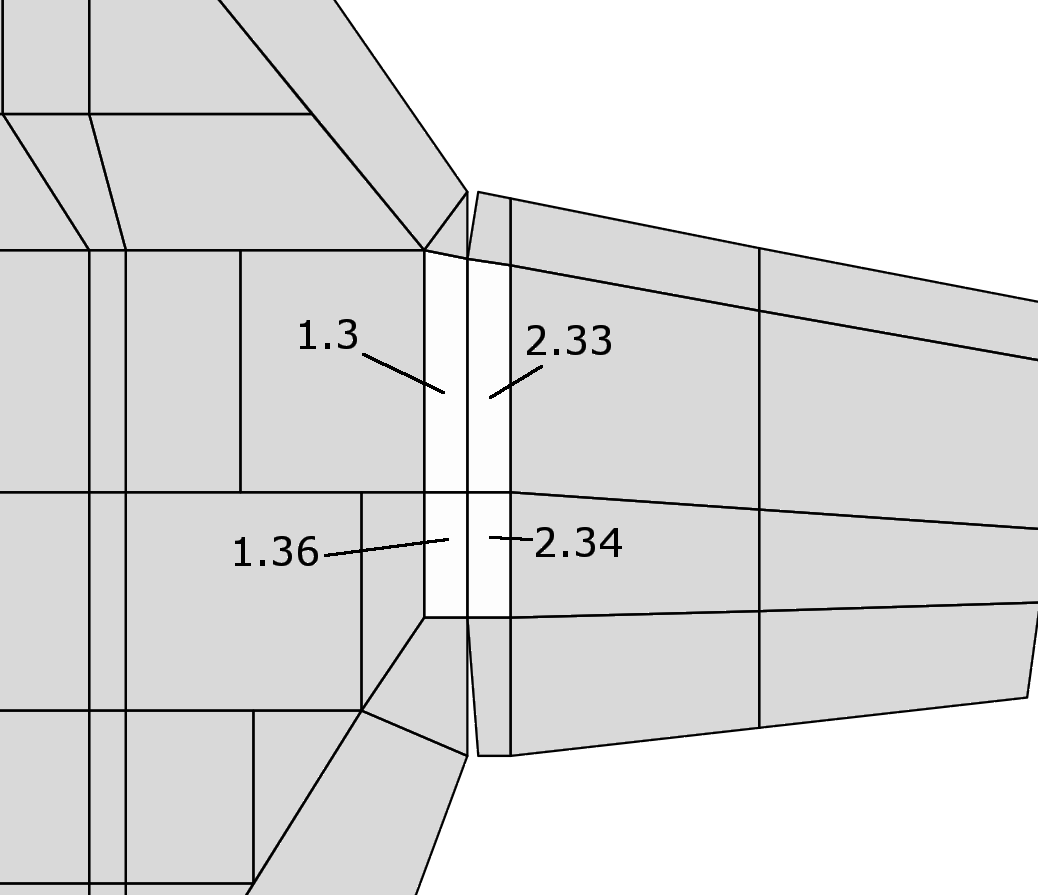
\includegraphics[width=0.5\textwidth]{RootOfWingWithSelectedPartsBW}
%\caption{Схематичное изображение вида сверху в месте стыка правого крыла и фюзеляжа}
%\label{fig:WingRootPlain}
%\end{figure}







На Рис.\ref{fig:stressToDiscreteness} представлены зависимости эквивалентных напряжений (напряжений по Мизесу) в выбранных точках от максимального размера для конечных элементов, используемых при построении модели (зависимости приведены для одного из вариантов конструкции). 

\begin{figure}[ht]
\centering
%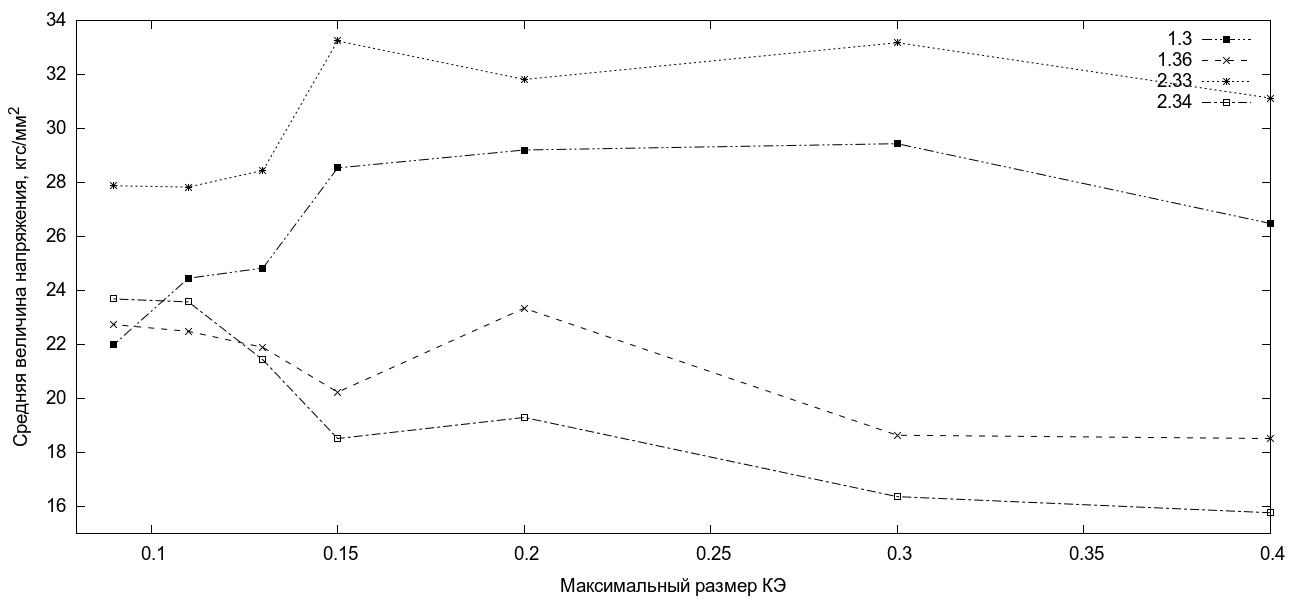
\includegraphics[width=0.8\textwidth]{StressToDiscretenessPlot}
\def\svgwidth{\textwidth}
% GNUPLOT: LaTeX picture with Postscript
\begingroup
  \makeatletter
  \providecommand\color[2][]{%
    \GenericError{(gnuplot) \space\space\space\@spaces}{%
      Package color not loaded in conjunction with
      terminal option `colourtext'%
    }{See the gnuplot documentation for explanation.%
    }{Either use 'blacktext' in gnuplot or load the package
      color.sty in LaTeX.}%
    \renewcommand\color[2][]{}%
  }%
  \providecommand\includegraphics[2][]{%
    \GenericError{(gnuplot) \space\space\space\@spaces}{%
      Package graphicx or graphics not loaded%
    }{See the gnuplot documentation for explanation.%
    }{The gnuplot epslatex terminal needs graphicx.sty or graphics.sty.}%
    \renewcommand\includegraphics[2][]{}%
  }%
  \providecommand\rotatebox[2]{#2}%
  \@ifundefined{ifGPcolor}{%
    \newif\ifGPcolor
    \GPcolorfalse
  }{}%
  \@ifundefined{ifGPblacktext}{%
    \newif\ifGPblacktext
    \GPblacktexttrue
  }{}%
  % define a \g@addto@macro without @ in the name:
  \let\gplgaddtomacro\g@addto@macro
  % define empty templates for all commands taking text:
  \gdef\gplbacktext{}%
  \gdef\gplfronttext{}%
  \makeatother
  \ifGPblacktext
    % no textcolor at all
    \def\colorrgb#1{}%
    \def\colorgray#1{}%
  \else
    % gray or color?
    \ifGPcolor
      \def\colorrgb#1{\color[rgb]{#1}}%
      \def\colorgray#1{\color[gray]{#1}}%
      \expandafter\def\csname LTw\endcsname{\color{white}}%
      \expandafter\def\csname LTb\endcsname{\color{black}}%
      \expandafter\def\csname LTa\endcsname{\color{black}}%
      \expandafter\def\csname LT0\endcsname{\color[rgb]{1,0,0}}%
      \expandafter\def\csname LT1\endcsname{\color[rgb]{0,1,0}}%
      \expandafter\def\csname LT2\endcsname{\color[rgb]{0,0,1}}%
      \expandafter\def\csname LT3\endcsname{\color[rgb]{1,0,1}}%
      \expandafter\def\csname LT4\endcsname{\color[rgb]{0,1,1}}%
      \expandafter\def\csname LT5\endcsname{\color[rgb]{1,1,0}}%
      \expandafter\def\csname LT6\endcsname{\color[rgb]{0,0,0}}%
      \expandafter\def\csname LT7\endcsname{\color[rgb]{1,0.3,0}}%
      \expandafter\def\csname LT8\endcsname{\color[rgb]{0.5,0.5,0.5}}%
    \else
      % gray
      \def\colorrgb#1{\color{black}}%
      \def\colorgray#1{\color[gray]{#1}}%
      \expandafter\def\csname LTw\endcsname{\color{white}}%
      \expandafter\def\csname LTb\endcsname{\color{black}}%
      \expandafter\def\csname LTa\endcsname{\color{black}}%
      \expandafter\def\csname LT0\endcsname{\color{black}}%
      \expandafter\def\csname LT1\endcsname{\color{black}}%
      \expandafter\def\csname LT2\endcsname{\color{black}}%
      \expandafter\def\csname LT3\endcsname{\color{black}}%
      \expandafter\def\csname LT4\endcsname{\color{black}}%
      \expandafter\def\csname LT5\endcsname{\color{black}}%
      \expandafter\def\csname LT6\endcsname{\color{black}}%
      \expandafter\def\csname LT7\endcsname{\color{black}}%
      \expandafter\def\csname LT8\endcsname{\color{black}}%
    \fi
  \fi
  \setlength{\unitlength}{0.0500bp}%
  \begin{picture}(8502.00,4534.00)%
    \gplgaddtomacro\gplbacktext{%
      \csname LTb\endcsname%
      \put(814,892){\makebox(0,0)[r]{\strut{} 16}}%
      \put(814,1267){\makebox(0,0)[r]{\strut{} 18}}%
      \put(814,1642){\makebox(0,0)[r]{\strut{} 20}}%
      \put(814,2017){\makebox(0,0)[r]{\strut{} 22}}%
      \put(814,2393){\makebox(0,0)[r]{\strut{} 24}}%
      \put(814,2768){\makebox(0,0)[r]{\strut{} 26}}%
      \put(814,3143){\makebox(0,0)[r]{\strut{} 28}}%
      \put(814,3518){\makebox(0,0)[r]{\strut{} 30}}%
      \put(814,3894){\makebox(0,0)[r]{\strut{} 32}}%
      \put(814,4269){\makebox(0,0)[r]{\strut{} 34}}%
      \put(1393,484){\makebox(0,0){\strut{} 0.1}}%
      \put(2512,484){\makebox(0,0){\strut{} 0.15}}%
      \put(3631,484){\makebox(0,0){\strut{} 0.2}}%
      \put(4749,484){\makebox(0,0){\strut{} 0.25}}%
      \put(5868,484){\makebox(0,0){\strut{} 0.3}}%
      \put(6986,484){\makebox(0,0){\strut{} 0.35}}%
      \put(8105,484){\makebox(0,0){\strut{} 0.4}}%
      \put(176,2486){\rotatebox{-270}{\makebox(0,0){\strut{}Средняя величина напряжения, $\text{кгс}/\text{мм}^2$}}}%
      \put(4525,154){\makebox(0,0){\strut{}Максимальный размер КЭ}}%
    }%
    \gplgaddtomacro\gplfronttext{%
      \csname LTb\endcsname%
      \put(7118,4096){\makebox(0,0)[r]{\strut{}$1.3$}}%
      \csname LTb\endcsname%
      \put(7118,3876){\makebox(0,0)[r]{\strut{}$1.36$}}%
      \csname LTb\endcsname%
      \put(7118,3656){\makebox(0,0)[r]{\strut{}$2.33$}}%
      \csname LTb\endcsname%
      \put(7118,3436){\makebox(0,0)[r]{\strut{}$2.34$}}%
    }%
    \gplbacktext
    \put(0,0){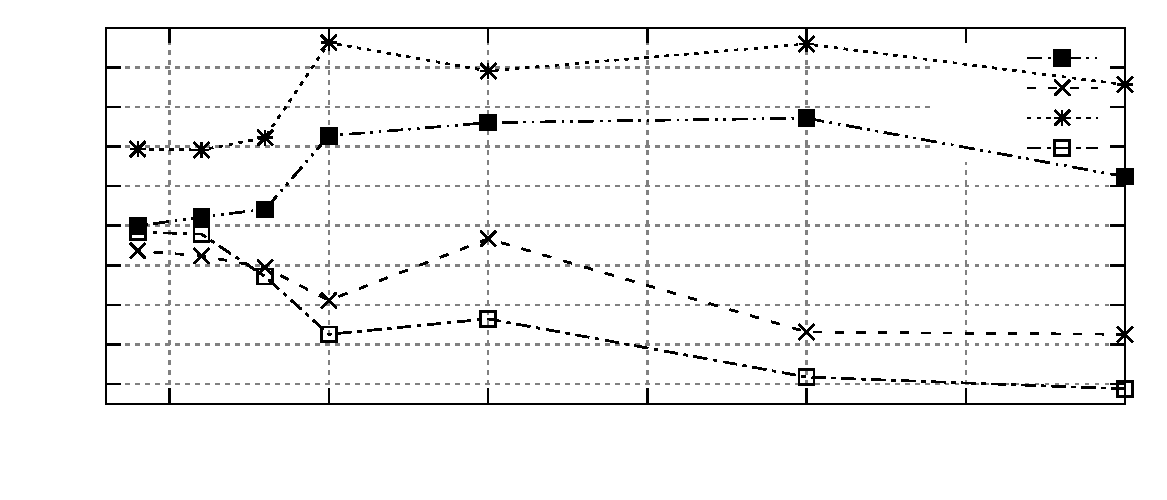
\includegraphics{StressToDiscreteness}}%
    \gplfronttext
  \end{picture}%
\endgroup

\caption{Зависимость напряжений в выбранных точках от максимальной величины КЭ, используемой в модели}
\label{fig:stressToDiscreteness}
\end{figure}


	

Исходя из полученных данных и с учетом зависимости трудоемкости процесса от максимального размера КЭ, была определена общая для всех трех вариантов конструкции рациональная величина конечного элемента ($0.11\m$) для дальнейших параметрических исследований моделей гипотетического БПЛА. 
%Ниже приведены картины НДС в месте стыка крыла с фюзеляжем при различных размерах конечного элемента. 


\section{Сравнение моделей}
\label{sec:modelsComparison}
Как было описано выше, в работе был проведен сравнительный анализ трех вариантов части конструкции, обеспечивающей крепление хвостовой части фюзеляжа к центроплану. Первый вариант представляет собой длинный узкий короб с несколькими перегородками (Рис.\ref{fig:variants_mke:1}). В этом варианте двигатель крепится в двух местах непосредственно к стенке короба. Данный вариант частично соответствует модельному варианту n стенок с $n = 4$, рассмотренному в разделе \ref{sec:pants}. Во втором варианте используется широкий плоский короб, частично расположенный над шассийной нишей (Рис.\ref{fig:variants_mke:2}). В данном варианте двигатель крепится к стенке короба и на боковое ребро короба. Третий вариант является промежуточным между первым и вторым и представляет собой широкий короб, соответствующий по высоте фюзеляжной части центроплана в месте их крепления (Рис.\ref{fig:variants_mke:3}). В данном варианте двигатель крепится аналогично второму варианту. 

Для каждого из исследуемых вариантов конструкции были определены рациональные параметры и вычислены весовые параметры. Ниже приведено сравнение относительных весовых характеристик моделей. Нумерация моделей в таблице соответствует нумерации на рисунках \ref{fig:variants_plain} и \ref{fig:variants_mke}

\tabulinesep = 1mm
\definecolor{lightgray}{gray}{0.9}
\begin{table}[H]
\captionsetup{justification=centering}
\caption{Таблица весовых характеристик моделей}
\begin{tabu}to \linewidth{*4{|X[m c]}|}
\hline
\taburowcolors {lightgray .. white}
 & Вариант 1 & Вариант 2 & Вариант 3 \\ \hline
%масса фюзеляжа & 850кг & 812кг  & 778кг \\ \hline
относительная масса фюзеляжа & $100\%$ & $95\%$ & $91,5\%$ \\ \hline
%масса обшивки & 489кг & 505кг  & 499кг \\ \hline
%масса подкрепляющего набора & 361кг & 307кг  & 277кг \\ \hline
\end{tabu}
\label{tab:variantsMasses}
\end{table}

Из полученных данных сделан вывод о том, что оптимальным по весовым характеристикам является использование третьего варианта конструкции.  

